\documentclass[11pt,blackandwhite]{beamer}
\usepackage[utf8x]{inputenc}

\definecolor{dalmostblack}{rgb}{.2,.2,.2}

\mode<presentation>
{
  %\usetheme{Rochester}
  \setbeamercovered{transparent}
  \setbeamercolor{normal text}{fg=dalmostblack,bg=lightgray}
  \setbeamercolor{alerted text}{fg=black}
  \setbeamercolor{example text}{fg=darkgray}
  \setbeamercolor{background canvas}{bg=white} 
  \setbeamercolor{structure}{fg=darkgray}

  \setbeamercolor{palette primary}{use=structure,fg=structure.fg}

  \setbeamercolor{math text}{}
  \setbeamercolor{math text inlined}{parent=math text}
  \setbeamercolor{math text displayed}{parent=math text}

  \setbeamercolor{normal text in math text}{}

  \setbeamercolor{local structure}{parent=structure}

  \setbeamercolor{titlelike}{parent=structure}

  \setbeamercolor{title}{parent=titlelike}
  \setbeamercolor{title in head/foot}{parent=palette quaternary}
  \setbeamercolor{title in sidebar}{parent=palette sidebar quaternary}

  \setbeamercolor{subtitle}{parent=title}

}
%\usepackage{ngerman}
%\usefonttheme{serif}
\newcommand{\page}[1]{\frame{#1}}

\usepackage{graphicx}
\usepackage{pstricks}
\usepackage{color}
\usepackage{listings}
\usepackage{amsmath}
\usepackage{amsfonts}
\usepackage{amssymb}
\usepackage{amsthm}
\usepackage{listings}
\usepackage{xspace}  % to allow for text macros that don't eat space 
\newcommand{\field}[1]{\mathbb{#1}}

\newtheorem{thm}{Theorem}[section]

\definecolor{dredcolor}{rgb}{.9,0.2,0.2}
\definecolor{blackcolor}{rgb}{0.0,0.0,0.0}
\definecolor{dgreencolor}{rgb}{0,0.4,0}
\definecolor{dbluecolor}{rgb}{.02,.02,.908}

\renewcommand{\emph}[1]{{\color{black}\bf #1}}

\newcommand{\SAGE}{{\color{blue}\sf Sage}\xspace}
\newcommand{\sage}{\SAGE}
\newcommand{\code}{\lstinline}


\title{How to get started with developing Sage}
%\author{Martin Albrecht}
% \institute{Information Security Group,\\
% Royal Holloway, University of London\\
% Egham, Surrey TW20 0EX, United Kingdom\\}

\institute{
\includegraphics[width=0.5\textwidth]{borg.jpg}}
%\titlegraphic{Seattle, 20. June 2008}
\date{Sage Days 16, Barcelona, June 23, 2009}

%\AtBeginSection[]
%{
%}

\lstdefinelanguage{Sage}[]{Python}
{morekeywords={True,False,sage},
sensitive=true}

\lstset{frame=none,
          showtabs=False,
          showspaces=False,
          showstringspaces=False,
          commentstyle={\color{dredcolor}\bfseries},
          keywordstyle={\color{black}\bfseries},
          stringstyle ={\color{darkgray}\bfseries},
          language = Sage,
          basicstyle={\tt}
          }

\begin{document}

\begin{frame}
\titlepage
\end{frame}

\begin{frame}
\frametitle{How to start developing Sage}
\begin{enumerate}
\item get tenure
\item ???
\item profit
\end{enumerate}
\end{frame}

\begin{frame}{Outline}
\tableofcontents
\begin{flushright}

\includegraphics[height=0.3\textwidth]{borg.jpg}
\end{flushright}
\end{frame}

\section{Why Would You Care?}
\begin{frame}
\frametitle{Outline}
\tableofcontents[sectionstyle=show/shaded]
\begin{flushright}

\includegraphics[height=0.3\textwidth]{picard.jpg}
\end{flushright}
\end{frame}

\begin{frame}
\frametitle{Enhancing Sage for your own research}
\begin{itemize}
\pause
 \item There is some bug which just plainly annoys you \dots \pause
 \item There is some function which just isn't documented properly and you
keep getting it wrong \dots \pause
 \item There is this functionality (which would be easy to add) but no
developer bothered \dots
\end{itemize}
 \pause
{
\begin{quote}
``It's easy, implement it and send me a patch.''
\end{quote}
\begin{flushright}
-- William Stein
\end{flushright}
}
\end{frame}

\begin{frame}
\frametitle{Writing your own non-trivial Sage programs} 
\begin{itemize}
 \item there isn't that much of a difference between developing for the Sage
core library and writing your own program.
 \item Most of the comments below apply to both.
 \item Please consider submitting your code to Sage if it implements
functionality not in Sage yet (or better than Sage)
\end{itemize}

\end{frame}


\begin{frame}
\frametitle{Using Sage as a frontend for your own library}
\begin{itemize}
 \item you wrote this amazing C/C++/whatever library and need to test it out
 \item you can either write tedious testcode or
 \item you can write a slim Sage interface which allows to test your library
much more rigorously.
 \item you can use this interface to convert between your native format and
many other systems (Pari, Magma, Mathematica, \dots)
\end{itemize}
\end{frame}

\begin{frame}
\frametitle{Let's face it} 

\begin{center}
You are stuck at this workshop anyway so you might as well write
some code while you are here. 
\end{center}


\end{frame}

\section{Overview}

\begin{frame}{Outline}
\tableofcontents[sectionstyle=show/shaded]
\begin{flushright}
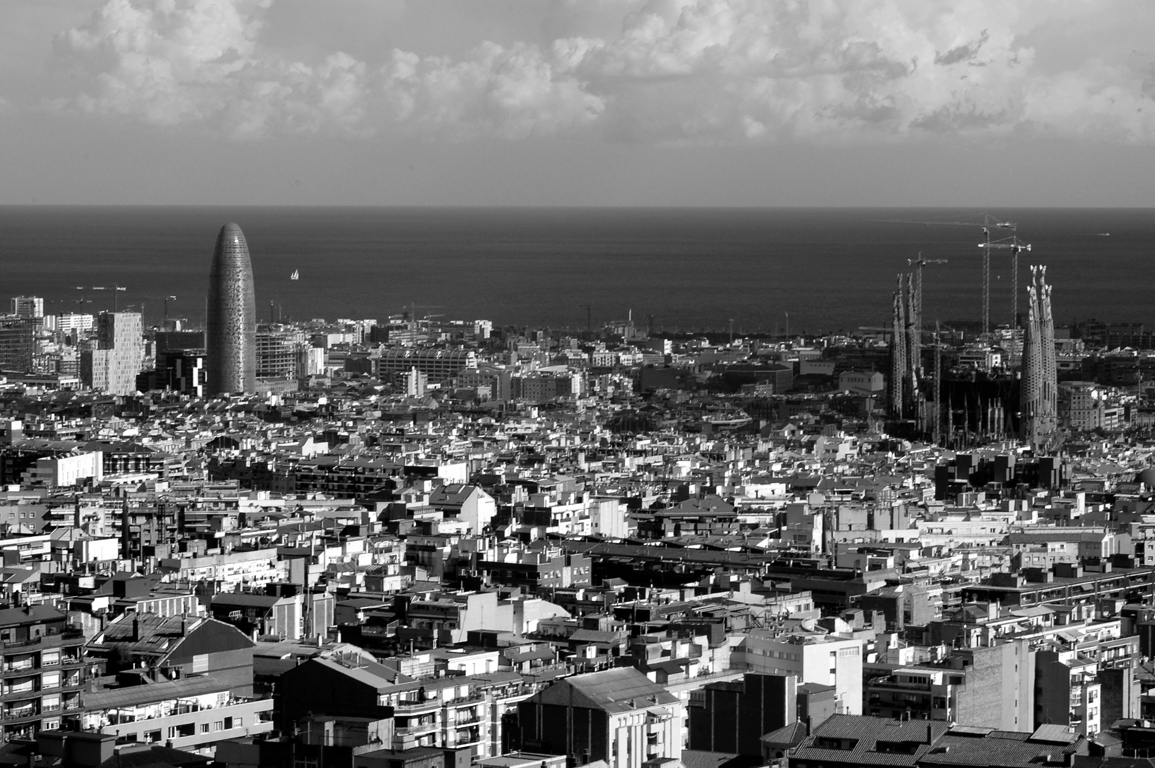
\includegraphics[height=0.3\textwidth]{overview.jpg}
\end{flushright}
\end{frame}

\begin{frame}
\frametitle{Python} 
\begin{figure}
 \centering
 
\includegraphics[width=0.5\textwidth]{python-and-cython.png}
 % python-and-cython.png: 678x118 pixel, 150dpi, 11.48x2.00 cm, bb=0 0 325 57
\end{figure}

\begin{itemize}
\item Sage fundamentally depends on Python.
\item Speaking Python is a requirement for properly using and developing Sage.
\item Python is a very easy to learn language.
\item Learning Python has benefits far beyond Sage, it is \emph{widely} used.
\end{itemize}

\begin{center}
 \url{http://www.diveintopython.org/} and\\
 \emph{Python in a Nutshell} by Alex Martelli
\end{center}
\end{frame}

\begin{frame}
\frametitle{Cython} 

\begin{figure}
 \centering
 
\includegraphics[width=0.5\textwidth]{python-and-cython.png}
 % python-and-cython.png: 678x118 pixel, 150dpi, 11.48x2.00 cm, bb=0 0 325 57
\end{figure}

Sage depends on Cython to provide

\begin{itemize}
 \item a compiled fast language for low-level arithmetic and
 \item a language to easily interface with C/C++ code and libraries.
\end{itemize}

If you want to work on this level, it makes sense to learn some Cython:

\begin{center}
 \url{http://docs.cython.org/}
\end{center}

\end{frame}

\begin{frame}[fragile]
\frametitle{The Preparser}
Sage commands get \emph{preparsed}.
\begin{itemize}
 \item \texttt{1/2} is \texttt{0} in Python, but \texttt{1/2} in Sage
 \item \texttt{P.<x,y> = GF(2)[]} is not valid Python, but valid in Sage
\end{itemize}

\begin{lstlisting}
sage: preparse("1/2")
'Integer(1)/Integer(2)'
sage: preparse("P.<x> = ZZ[]")
"P = ZZ['x']; (x,) = P._first_ngens(1)"
sage: preparse("0.5")
"RealNumber('0.5')"
\end{lstlisting}

When writing code for the Sage Library you must write valid Python and you have
to expect Python behaviour (e.g. \texttt{1/2 == 0}).
\end{frame}

\begin{frame}
\frametitle{Components}
\begin{itemize}
 \item Sage comes in various SPKGs: Sage Packages.
 \item Sage 4.0.1 contains 99 such SPKGs like bzip2, MPIR, Pari, NTL, FLINT,
Maxima, Singular etc.
 \item This way Sage is self contained and behaves reasonably similar across
platforms.
 \item The code which ties all these packages together is the ``\emph{Sage
Library}''. Naturally, it comes in an SPKG.
 \item Each copy of Sage allows you to hack the Sage Library straight away --
batteries included.
\end{itemize}

I will focus on modifying the Sage Library in this talk.
\end{frame}

\begin{frame}
\frametitle{Directory structure}
\texttt{\$SAGE\_ROOT}
\begin{description}
 \item[\texttt{local}] where the SPKGs are installed to
  \begin{description}
   \item[\texttt{bin}] executables go here (e.g. \texttt{Singular})
   \item[\texttt{lib}] e.g. shared libraries go here (e.g.
\texttt{libsingular.so})
  \end{description}
 \item[\texttt{devel/sage}] the Sage Library
 \begin{description}
 \item[\texttt{doc}] the reference manual, tutorial etc. sources
 \item[\texttt{sage}] the code that makes things happen
 \item[\texttt{c\_lib}] some low-level code, can be ignored by most
 \end{description}
 \item[\texttt{spkgs}] this is where the SPKGs are stored
\end{description}
\end{frame}

\begin{frame}
\frametitle{Directory structure of the Sage library}
Excerpt:
\begin{small}
\begin{tabular}{|r|r|}
\hline
algebras & free, group, quaternion, steenrod \dots \\
combinat & very comprehensive combinatorics\\
graphs & all things graph theory\\
groups & group theory\\
interfaces & interfaces to other system (e.g. Magma)\\
libs & raw interfaces to C/C++ libraries\\
matrix & matrices over all kinds of fields\\
misc & a lot of useful utility functions!\\
modular & modular forms and symbols\\
plot & 2d and 3d plotting\\
quadratic\_forms & guess what.\\
rings & integers, rationals, finite fields, polynomials, $p$-adics\\
schemes & curves (e.g. elliptic, hyperelliptic)\\
server & the notebook server\\
structure & coercion and Sage parent--element infrastructure\\
symbolic & all things symbolic manipulation\\
\hline
\end{tabular}
\end{small}
\end{frame}


\begin{frame}[allowframebreaks,fragile]

\frametitle{Finding that function}

\begin{scriptsize}
\begin{lstlisting}
sage: search_src("Integer","create")
...
misc/preparser.py:We create a raw integer.
misc/preparser.py:first one computes a list of SAGE integers ...
monoids/free_monoid.py:        One can create a free monoid  ...
combinat/sf/sfa.py:           integer n as its input and  ...
server/notebook/js.py:                            string  ...
matrix/matrix2.pyx:        We create the zero matrix over...
misc/parser.pyx:variables) and how integer and floating ...
rings/integer.pyx:        You can create an integer from ...
rings/integer.pyx: A global  pool for performance when  ...
rings/integer.pyx:   if available, otherwise a new Integer ...
rings/integer_ring.pyx:To create an ``Integer``, coerce  ...
rings/integer_ring.pyx:    We can create integers from ...
...
\end{lstlisting}
\end{scriptsize}

\framebreak

\begin{scriptsize}
\begin{lstlisting}
sage: search_def("rank")
algebras/free_algebra_quotient.py:    def rank(self):
combinat/choose_nk.py:    def rank(self, x):
...
combinat/subset.py:    def rank(self, sub):
misc/functional.py:def rank(x):
modules/free_module.py:    def rank(self):
modules/matrix_morphism.py:    def rank(self):
combinat/posets/hasse_diagram.py:    def rank(self,element=None):
...
combinat/words/alphabet.py:    def rank(self, letter):
libs/mwrank/interface.py:    def rank(self):
modular/abvar/abvar.py:    def rank(self):
...
modular/modsym/ambient.py:    def rank(self):
quadratic_forms/genera/genus.py:    def rank(self):
...
matrix/matrix0.pyx:    def rank(self):
matrix/matrix_integer_dense.pyx:    def rank(self):
matrix/matrix_mod2_dense.pyx:    def rank(self):
matrix/matrix_modn_dense.pyx:    def rank(self):
matrix/matrix_modn_sparse.pyx:    def rank(self, gauss=False):
matrix/matrix_rational_dense.pyx:    def rank(self):
...
\end{lstlisting}
\end{scriptsize}

\framebreak

\code{edit()} tries hard to an editor at the right line in the right file
\texttrademark.

\begin{scriptsize}
\begin{lstlisting}
sage: edit(ZZ)
cdef class IntegerRing_class(PrincipalIdealDomain):
    r"""
    The ring of integers.

    In order to introduce the ring `\ZZ` of integers, we
    illustrate creation, calling a few functions, and 
    working with its elements.
    ...
\end{lstlisting}
\end{scriptsize}

\framebreak

\begin{tiny}
\begin{lstlisting}
sage: ZZ??
Type:       IntegerRing_class
Base Class: <type 'sage.rings.integer_ring.IntegerRing_class'>
String Form:Integer Ring
Namespace:  Interactive
File: .../local/lib/python2.5/site-packages/sage/rings/integer_ring.so
Docstring:

        The ring of integers.

        In order to introduce the ring `ZZ` of integers, we
        illustrate creation, calling a few functions, and working with its
        elements.

\end{lstlisting}
\end{tiny}

\begin{itemize}
 \item \texttt{sage.rings.integer\_ring.IntegerRing\_class}
 \item \texttt{.../site-packages/sage/rings/integer\_ring.so}
\end{itemize}
$\longrightarrow$
\texttt{\$SAGE\_ROOT/devel/sage/\emph{sage/rings/integer\_ring.pyx}}
\end{frame}

\begin{frame}
\frametitle{site-packages vs. devel}
\begin{itemize}
 \item on the last slide the source file for \texttt{ZZ} was given as
{\scriptsize\texttt{
local/lib/python2.5/site-packages/sage/rings/integer\_ring.so }}
 \item this is where the code that is actually run is stored
 \item the sources are in \texttt{devel/sage/sage/rings/integer\_ring.pyx}
 \item the command \emph{sage -b} compiles and copies the sources for you
\end{itemize}

Always edit the files in the \texttt{devel} subdirectory and call \emph{sage
-b} to (compile and) copy them over.
\end{frame}

\begin{frame}[fragile, allowframebreaks]
\frametitle{Built-in documentation}
\begin{tiny}
\begin{lstlisting}
sage: ZZ?
... 
        The ring of integers.

        In order to introduce the ring `ZZ` of integers, we
        illustrate creation, calling a few functions, and working with its
        elements.

        ::

            sage: Z = IntegerRing(); Z
            Integer Ring
            sage: Z.characteristic()
            0
            sage: Z.is_field()
            False

        We next illustrate basic arithmetic in `ZZ`::

            sage: a = Z(1234); b = Z(5678); print a, b
            1234 5678
...
\end{lstlisting}
\framebreak
\begin{lstlisting}
sage: help(ZZ)
 Help on IntegerRing_class object:

class IntegerRing_class(sage.rings.ring.PrincipalIdealDomain)
 |  File: sage/rings/integer_ring.pyx (starting at line 104)
 |
 |  The ring of integers.
 |
 |  In order to introduce the ring `\ZZ` of integers, we
 |  illustrate creation, calling a few functions, and working with its
 |  elements.
 |
 |  ::
 |
 |      sage: Z = IntegerRing(); Z
 |      Integer Ring
 |      sage: Z.characteristic()
 |      0
 |      sage: Z.is_field()
 |      False
...
\end{lstlisting}
\end{tiny}
\end{frame}

\begin{frame}[fragile]
\frametitle{Source code}
\begin{tiny}
\begin{lstlisting}
sage: ZZ?? 
...
   def __init__(self):
        ParentWithGens.__init__(self, self, ('x',), normalize=False)
        self._populate_coercion_lists_(element_constructor=integer.Integer,
                                       init_no_parent=True,
                                       convert_method_name='_integer_')

    def __cinit__(self):
        # This is here because very old pickled integers ...
        global number_of_integer_rings
        if type(self) is IntegerRing_class:
            if number_of_integer_rings > 0:
              self._populate_coercion_lists_(\
                     element_constructor=integer.Integer, \
                     init_no_parent=True, \
                     convert_method_name='_integer_')
            number_of_integer_rings += 1

    def __reduce__(self):
        """
        TESTS::

            sage: loads(dumps(ZZ)) is ZZ
            True
        """
        return IntegerRing, ()

...
\end{lstlisting}
\end{tiny}
\end{frame}

\begin{frame}[allowframebreaks]
\frametitle{Writing documentation}
\begin{itemize}
 \item Every function or class added to Sage \emph{must} have documentation of
its functionality and inputs.
 \item Sage docstrings are formated using the ReStructuredText.
\end{itemize}

Build the reference manual by typing \texttt{sage -b} first and then
\texttt{sage -docbuild reference html} and check

\begin{itemize}
 \item that it produces no errors and
 \item that the HTML looks okay.
\end{itemize}

\framebreak

\emph{Examples}
\begin{itemize} 
 \item \code{*foo*}: \textit{foo}
 \item \code{**foo**}: \textbf{foo}
 \item \code{``x^i``}: \texttt{verbatim environment}
 \item \code{`x^i`}: \LaTeX\ math mode $x^i$
 \item Any line ending with \texttt{::} means that the following indented
things are a literal block (usually \texttt{sage: commands})
\end{itemize}

See 

\begin{center}
\url{http://www.sagemath.org/doc/developer/sage_manuals.html}
\end{center}

for more details.

\end{frame}

\begin{frame}[fragile, allowframebreaks]
\frametitle{Running tests}
\begin{itemize}
 \item Every new function included with Sage \emph{must} have doctests.
 \item doctests are examples on how to use a function and are run on a regular
basis to test for regressions.
\end{itemize}
\begin{tiny}
\begin{lstlisting}
sage: e.log?
EXAMPLES::

    sage: Integer(124).log(5)
    sage: Integer(125).log(5)
    3
    sage: Integer(125).log(5,prec=53)
    3.00000000000000
    sage: log(Integer(125))
    log(125)

For extremely large numbers, this works::

    sage: x = 3^100000
\end{lstlisting}
\end{tiny}
For tests which are not end-user friendly use \code{TESTS::}.

\framebreak

\begin{itemize}
 \item You can run doctests on a single file as 
\code{sage -t filename_or_directory}.
 \item You can run doctests in parallel as 
\code{sage -tp num_threads filename_or_directory}
 \item You can and should also add and run doctests on your private code to
test for regressions in Sage and/or your code.
 \item Before submitting a patch to Trac you should run doctests on the
complete Sage tree (\code{make test}).
 \item If your computer is too slow for this, ask William about an account on
\url{http://sage.math.washington.edu}.
\end{itemize}
\end{frame}

\section{Revision Control}
\begin{frame}{Outline}
\tableofcontents[sectionstyle=show/shaded]
\begin{flushright}

\includegraphics[height=0.3\textwidth]{mercurial.png}
\end{flushright}
\end{frame}

\begin{frame}
\frametitle{Mercurial}
Mercurial is the source control system that is used with Sage. 

\begin{center}

\includegraphics[height=0.2\textwidth]{mercurial-logo.png}
\end{center}

See
\begin{center}
\url{http://www.selenic.com/mercurial/}  
\end{center}
for full documentation on Mercurial.
\end{frame}

\begin{frame}[fragile]
\frametitle{Batteries included}
All of the Mercurial repositories related to Sage are included with
Sage. Thus the complete change history and setup for doing
development is available in your copy of Sage.

\vspace{1em}

Before using Mercurial, make sure to define your username so the
patches you make are identified as yours. Make a file \verb|~/.hgrc|
in your home directory like this one:

\begin{lstlisting}
[ui]
username = John Doe <doe@example.com>

[extensions]
hgext.mq =
\end{lstlisting}
\end{frame}

\begin{frame}
\frametitle{Running \code{Hg}}

There are several ways to run Mercurial: 
\begin{itemize}
 \item from the command line, run \code{sage -hg} (\code{Hg} is the chemical
symbol for mercury), 
 \item or from within Sage, run \code{hg\_sage}. Most of the examples below use
the second method.
\end{itemize}

Before you modify Sage library files, you might want to create a
copy of the Sage library in which to work. 

\vspace{1em}

Do this by typing
\code{sage -clone myver}, for example; then Sage will use
Mercurial to clone the current repository and call the result
\code{myver}.

\vspace{1em}

You can switch between copies by \code{sage -b main} and \code{sage -b myver}.
\end{frame}

\begin{frame}
\frametitle{Building changed source files}
Once you have copied the library to a new branch \code{myver} and
edited some files there, you should build the Sage library to
incorporate those changes: type \code{sage -b myver}, or just
\code{sage -b} if the branch \code{myver} is already the
current branch: that is, if \code{SAGE\_ROOT/devel/sage} links
to \code{SAGE\_ROOT/devel/sage-myver}.

\vspace{1em}

Note that \code{devel/sage} is a symlink to whatever branch/clone is currently
``active.''

\vspace{1em}

You can also type \code{sage -br myver} to build the library and then to
immediately run Sage.
\end{frame}

\begin{frame}
\frametitle{How to revert changes}
\begin{itemize}
 \item If you did \code{sage -clone myver} you can simply \code{sage -b main} to
return to the upstream version of Sage
 \item You can also enter \code{hg_sage.revert()} to undo uncommitted changes.
 \item You can use \code{hg_sage.update()} to return to a previous revision to
``undo'' committed changes.
\end{itemize}
 
\end{frame}


\begin{frame}[allowframebreaks]
\frametitle{Preparing patches}
If you want to submit your changes to the Sage development team for
refereeing (and inclusion into Sage if the referee's report is
positive), you should produce patch files. 

To do this:
\begin{itemize}
\item Type \code{hg\_sage.status()} and \code{hg\_sage.diff()}
to see exactly what you've done (you can pass options to
\code{diff} to see information about certain files).

\item If you've added new files, not just edited existing ones, type
\code{hg\_sage.add({[}filenames{]})} to add those new files to your
repository.
\framebreak

\item Commit your changes by typing
\code{hg\_sage.commit({[}optional filenames{]})} to commit the
changes in files to the repository -- if no filenames are given,
all files are committed. First the output of \code{hg diff} is
displayed: look at it or just enter \code{q}. Then you are
dumped into an editor to type a brief comment on the changes. The
default editor is vi, so type \code{i}, write some meaningful
one line description, hit \code{Escape} and type \code{:wq}.

(In bash, to make emacs the default editor, type \code{export EDITOR=emacs}.)

\framebreak

\item Now create a patch file using \code{hg\_sage.export(...)}.
This command needs a revision number (or list of revision numbers)
as an argument; use \code{hg\_sage.log()} to see these numbers.
An optional second argument to \code{hg\_sage.export(...)} is a
filename for the patch; the default is
\code{(changeset\_revision\_number).patch}.

\item Then post your patch on the Sage Trac server (see below).
\end{itemize}
\end{frame}

\begin{frame}
\frametitle{Other stuff}
Finally, if you want to apply a patch file (perhaps you've
downloaded a patch from the Trac server for review), use the
command \code{hg\_sage.patch('filename')}.

\vspace{1em}
Most Sage developers seem to use a Mercurial extension called Mercurial Queues
these days to manage their patches. See
\begin{center}
\url{http://www.selenic.com/mercurial/wiki/MqExtension} \\
\url{http://wiki.sagemath.org/MercurialQueues}
\end{center}
for details.
\end{frame}



\section{The Sage Development Process}
\begin{frame}{Outline}
\tableofcontents[sectionstyle=show/shaded]
\begin{flushright}
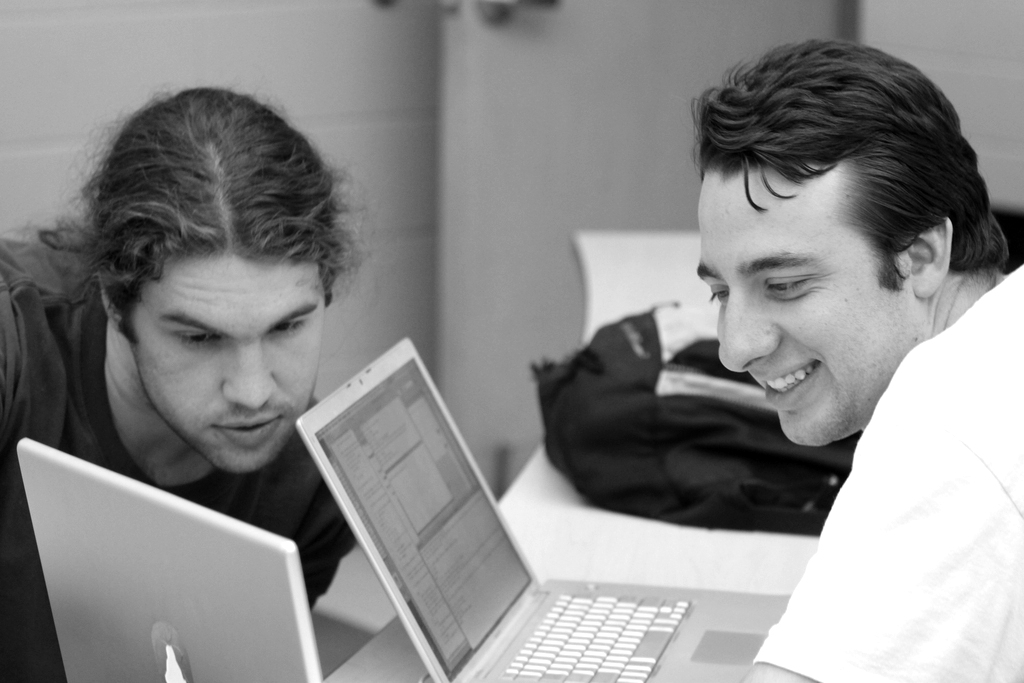
\includegraphics[height=0.3\textwidth]{process.jpg}
\end{flushright}
\end{frame}

\begin{frame}[allowframebreaks]
\frametitle{How Alice gets code into Sage}

 \begin{figure}
 \centering
 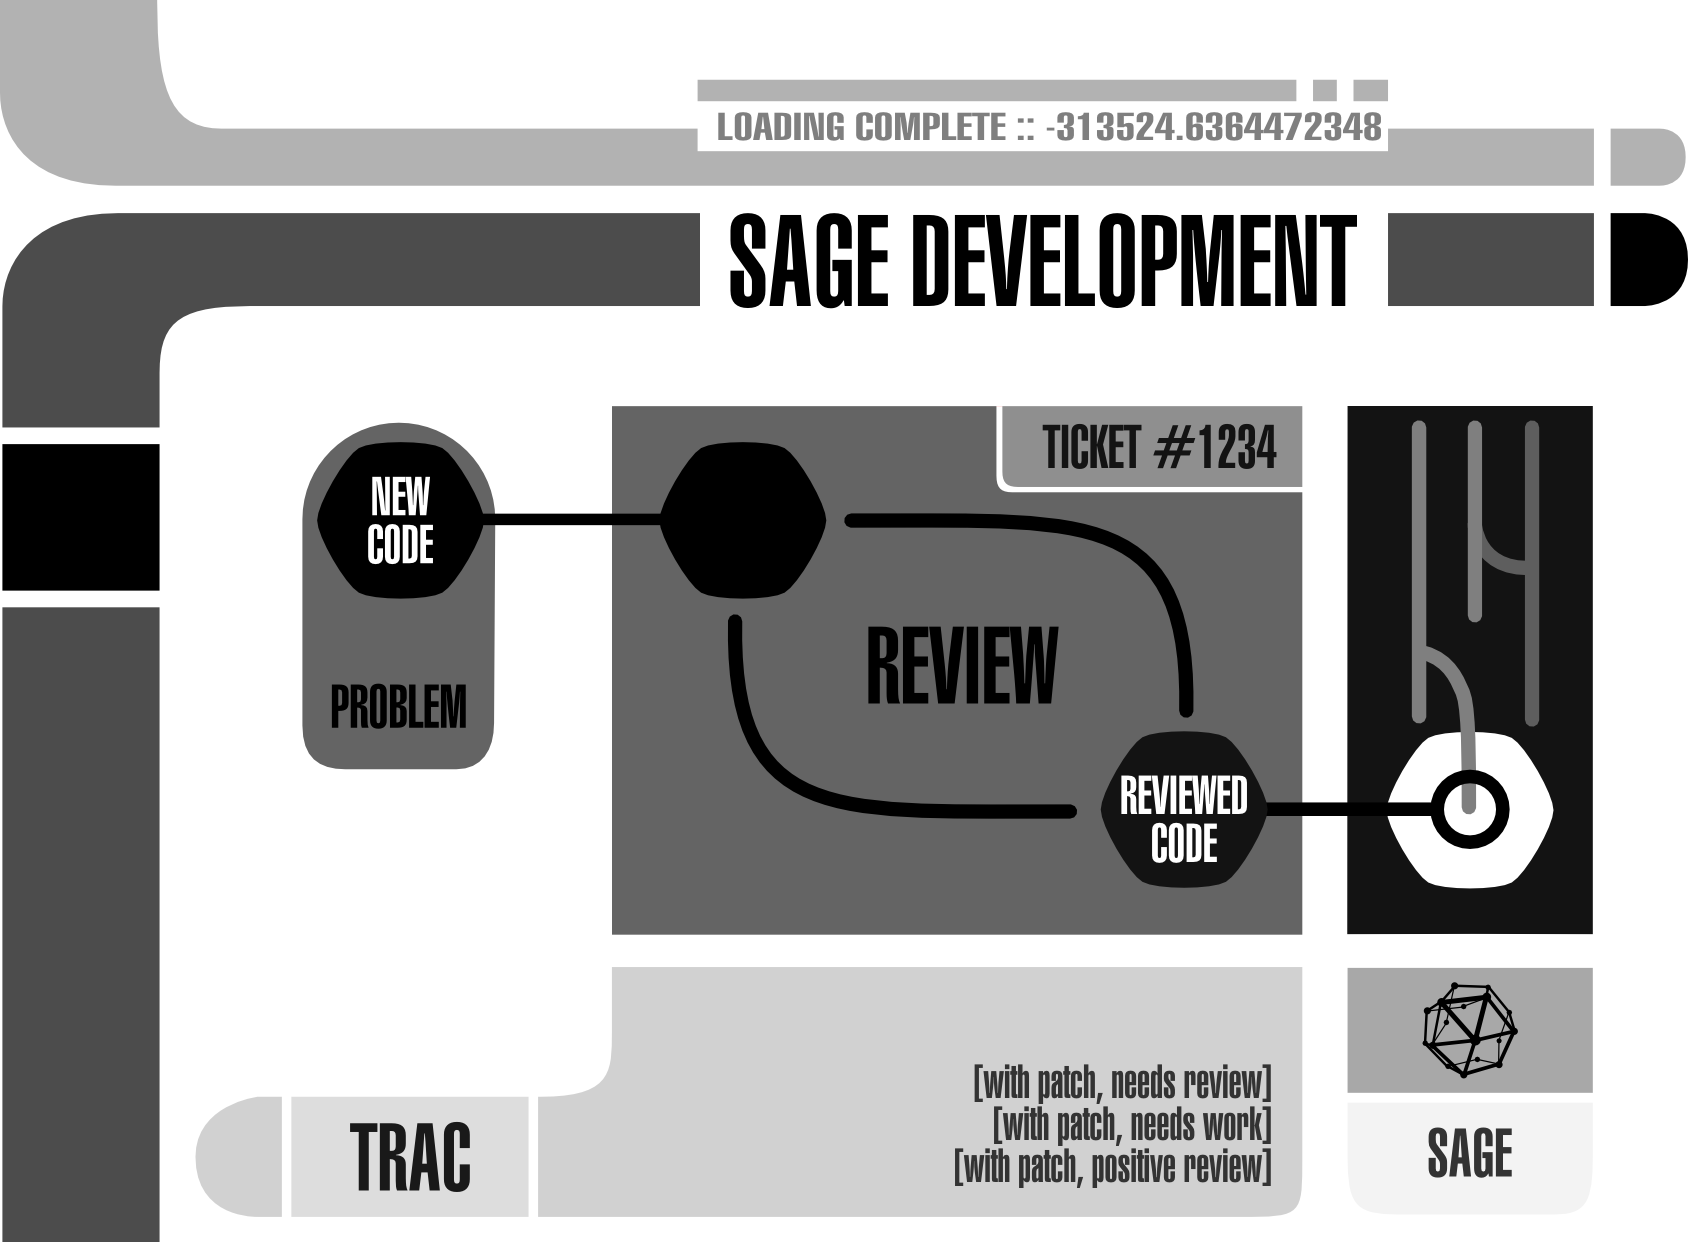
\includegraphics[width=0.95\textwidth]{sage-development.png}
 % sage-development.png: 1147x830 pixel, 100dpi, 29.13x21.08 cm, bb=0 0 826 598
\end{figure}

\framebreak

\begin{enumerate}
 \item Alice writes some awesome code, opens a trac ticket at
\url{http://trac.sagemath.org} and attaches her patch. The subject line of the
ticket is now: \texttt{[with patch, needs review] \dots}
 \item Bob reviews Alice's patch and finds an issue. The subject line
of the ticket is now: \texttt{[with patch, needs work] \dots}
\item Alice fixes the issues, Bob checks the changes and decides it is okay
now: \texttt{[with patch, positive review]}.
\item Eve is acting release manager for Sage X.Y.Z and applies Alice's
patch to her tree. If everything is fine she closes the ticket, otherwise the
ticket gets \texttt{[with patch, needs work]}.
\end{enumerate}

\end{frame}



\begin{frame}
\frametitle{Requesting a Trac Account}
\begin{itemize}
\item To prevent Spam, we have had to disable anonymous creation and
editing of tickets.
\item  Please write an email to wstein@gmail.com and provide an
account name and password. 
\item The account name should be non-silly, i.e. no first names, no
leet-handles.
\end{itemize}
\end{frame}

\begin{frame}
\frametitle{Opening Tickets}
Tickets can either be opened to submit a patch or to request a bugfix or
enhancement.

\begin{itemize}
 \item Before opening a ticket, make sure that nobody else has opened a ticket
about the same or closely related issue. 
 \item It is better to open several specific tickets than one that is very
broad. 
 \item Be precise: If foo doesn't work on OSX, but is fine on Linux, mention
that in the title. Also use the keyword option to make searches pick up the
issue. 
\end{itemize}
\end{frame}

\begin{frame}
\frametitle{Finding someone to review your patch} 
\begin{itemize}
 \item Components on Trac have defaults assigned, so hopefully that will take
care of it already.
 \item If you know someone who can review your patches, it makes sense to ask
directly.
 \item If you are fixing a bug in/adding documentation to \code{sage -hg
annotate -u filename} is a good tool to identify who wrote that function.
 \item You can ask the release manager or on [sage-devel] to find someone to
review your patch.
\end{itemize}

\end{frame}


\begin{frame}
\frametitle{Reviewing Patches}
\begin{itemize}
\item The code makes sense and reads okay.
\item 100\% doctests: All new code must be 100\% doctested. \emph{There is no
way around this.} 

\item Bug fixes must be doctested: The patch that fixes an issue must also
contain a doctest specifically to test the problem. This is not always possible,
so this is not enforced in certain situations. 

\item Test the reference manual: \texttt{sage -docbuild reference html} must
produce no errors 

\item Test the Sage Library: \texttt{make test} or \texttt{make ptest} (edit
number of threads in
makefile before using ptest!)
\end{itemize}

\end{frame}


\section{The Sage Community}

\begin{frame}{Outline}
\tableofcontents[sectionstyle=show/shaded]
\begin{flushright}
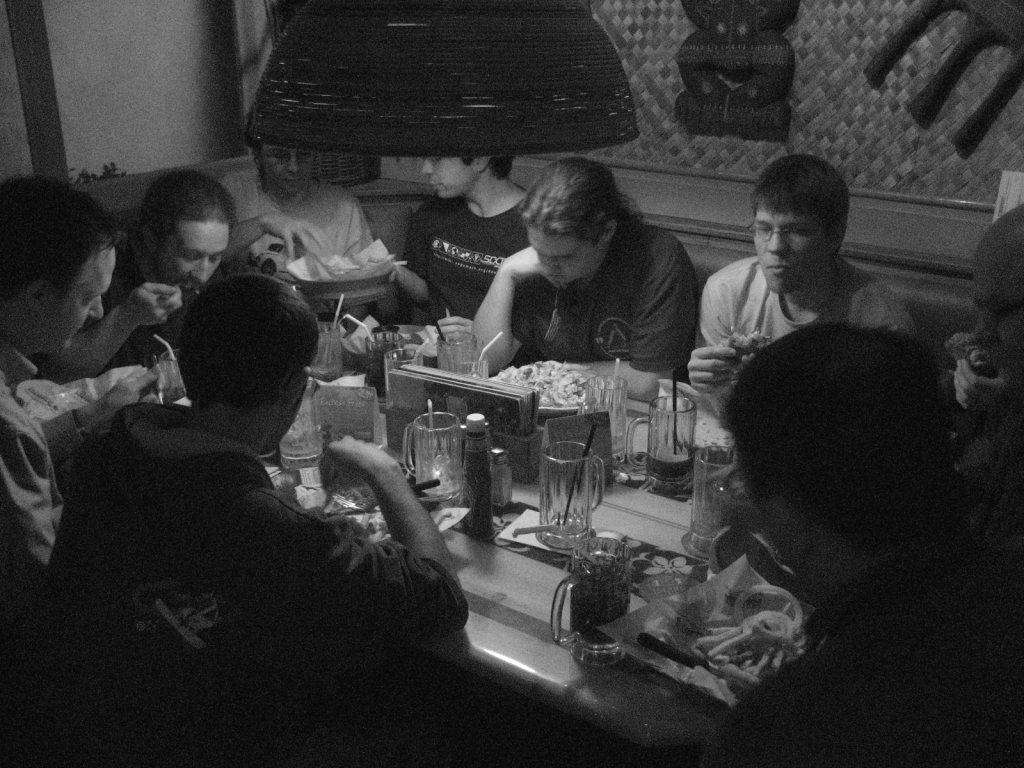
\includegraphics[height=0.3\textwidth]{community.jpg}
\end{flushright}
\end{frame}

\begin{frame}
\frametitle{Asking Questions} 

Definitely do ask a lot of questions!

\begin{description}
 \item[sage-devel] the main development list: 900 members, 1000 messages
per month
 \item[sage-support] end-user support list: 1220 members, 800 messages per
month 
 \item[\#sage-devel] on freenode: main development IRC channel, 30 members,
medium activity, usually at least two `core' developers around
 \item[real people] this might be a good moment for the Sage developers in the
room to stand up and introduce themselves.
\end{description}
\end{frame}

\begin{frame}
\frametitle{Netiquette}
\begin{itemize}
 \item Many Sage developers are volunteers and have day jobs or other
obligations.
 \item Usually, questions are answered quickly if someone knows the answer
straight away.
 \item If your question goes unanswered, it is probably just because people
didn't get around to it yet. Don't hesitate to ask again!
 \item Keep it friendly though, we take pride in the fact that our mailing lists
hardly see any insults and flame wars.
\end{itemize}
 
\end{frame}


\begin{frame}
\frametitle{Other Resources}
\begin{itemize}
 \item The wiki (\url{http://wiki.sagemath.org}) a wonderful collection of
useful outdated information.
 \item The developer guide (\url{http://www.sagemath.org/doc/developer/})
should contain everything to get started, if not \emph{write it and send us a
patch!} or let us know at least.
 \item The archive of [sage-devel]
(\url{http://groups.google.com/group/sage-devel}) contains tons of useful
information.
\end{itemize}
 
\end{frame}



\begin{frame}{Thank You!}
\begin{center}
 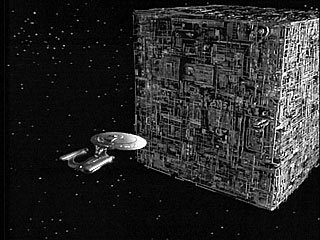
\includegraphics[width=0.4\textwidth]{cube.jpg}\\
\begin{quote}
Building the Cube instead of reinventing the Warp drive!
\end{quote}

 % xorrox.jpg: 1024x768 pixel, 72dpi, 36.12x27.09 cm, bb=0 0 1024 768
\end{center}

\end{frame}


% \begin{frame}[allowframebreaks]
% \bibliographystyle{plain}
% \bibliography{../../literature}
% \end{frame}

\end{document}

